\documentclass[10pt,ignorenonframetext,,aspectratio=149]{beamer}
\usefonttheme{serif} % use mainfont rather than sansfont for slide text
\setbeamertemplate{caption}[numbered]
\setbeamertemplate{caption label separator}{: }
\setbeamercolor{caption name}{fg=normal text.fg}
\usepackage{lmodern}
\usepackage{amssymb,amsmath}
\usepackage{ifxetex,ifluatex}
\usepackage{fixltx2e} % provides \textsubscript
\ifnum 0\ifxetex 1\fi\ifluatex 1\fi=0 % if pdftex
  \usepackage[T1]{fontenc}
  \usepackage[utf8]{inputenc}
\else % if luatex or xelatex
  \ifxetex
    \usepackage{mathspec}
  \else
    \usepackage{fontspec}
  \fi
  \defaultfontfeatures{Ligatures=TeX,Scale=MatchLowercase}
  \newcommand{\euro}{€}
    \setmainfont[]{Open Sans}
\fi
% use upquote if available, for straight quotes in verbatim environments
\IfFileExists{upquote.sty}{\usepackage{upquote}}{}
% use microtype if available
\IfFileExists{microtype.sty}{%
\usepackage{microtype}
\UseMicrotypeSet[protrusion]{basicmath} % disable protrusion for tt fonts
}{}
\usepackage{graphicx,grffile}
\makeatletter
\def\maxwidth{\ifdim\Gin@nat@width>\linewidth\linewidth\else\Gin@nat@width\fi}
\def\maxheight{\ifdim\Gin@nat@height>\textheight0.8\textheight\else\Gin@nat@height\fi}
\makeatother
% Scale images if necessary, so that they will not overflow the page
% margins by default, and it is still possible to overwrite the defaults
% using explicit options in \includegraphics[width, height, ...]{}
\setkeys{Gin}{width=\maxwidth,height=\maxheight,keepaspectratio}

% Comment these out if you don't want a slide with just the
% part/section/subsection/subsubsection title:
\AtBeginPart{
  \let\insertpartnumber\relax
  \let\partname\relax
  \frame{\partpage}
}
\AtBeginSection{
  \let\insertsectionnumber\relax
  \let\sectionname\relax
  \frame{\sectionpage}
}
\AtBeginSubsection{
  \let\insertsubsectionnumber\relax
  \let\subsectionname\relax
  \frame{\subsectionpage}
}

\setlength{\emergencystretch}{3em}  % prevent overfull lines
\providecommand{\tightlist}{%
  \setlength{\itemsep}{0pt}\setlength{\parskip}{0pt}}
\setcounter{secnumdepth}{0}

\title{Endogeneity and Instrumental Variables Estimation}
\author{Henrique Veras}
\date{}

%% Here's everything I added.
%%--------------------------

\usepackage{graphicx}
\usepackage{rotating}
%\setbeamertemplate{caption}[numbered]
\usepackage{hyperref}
\usepackage{caption}
\usepackage[normalem]{ulem}
%\mode<presentation>
\usepackage{wasysym}
%\usepackage{amsmath}


% Get rid of navigation symbols.
%-------------------------------
\setbeamertemplate{navigation symbols}{}

% Optional institute tags and titlegraphic.
% Do feel free to change the titlegraphic if you don't want it as a Markdown field.
%----------------------------------------------------------------------------------
\institute{PIMES/UFPE}

% \titlegraphic{\includegraphics[width=0.3\paperwidth]{\string~/Dropbox/teaching/clemson-academic.png}} % <-- if you want to know what this looks like without it as a Markdown field. 
% -----------------------------------------------------------------------------------------------------


% Some additional title page adjustments.
%----------------------------------------
\setbeamertemplate{title page}[empty]
%\date{}
\setbeamerfont{subtitle}{size=\small}

\setbeamercovered{transparent}

% Some optional colors. Change or add as you see fit.
%---------------------------------------------------
\definecolor{clemsonpurple}{HTML}{522D80}
 \definecolor{clemsonorange}{HTML}{F66733}
\definecolor{uiucblue}{HTML}{003C7D}
\definecolor{uiucorange}{HTML}{F47F24}


% Some optional color adjustments to Beamer. Change as you see fit.
%------------------------------------------------------------------
\setbeamercolor{frametitle}{fg=clemsonpurple,bg=white}
\setbeamercolor{title}{fg=clemsonpurple,bg=white}
\setbeamercolor{local structure}{fg=clemsonpurple}
\setbeamercolor{section in toc}{fg=clemsonpurple,bg=white}
% \setbeamercolor{subsection in toc}{fg=clemsonorange,bg=white}
\setbeamercolor{footline}{fg=clemsonpurple!50, bg=white}
\setbeamercolor{block title}{fg=clemsonorange,bg=white}


\let\Tiny=\tiny


% Sections and subsections should not get their own damn slide.
%--------------------------------------------------------------
\AtBeginPart{}
\AtBeginSection{}
\AtBeginSubsection{}
\AtBeginSubsubsection{}

% Suppress some of Markdown's weird default vertical spacing.
%------------------------------------------------------------
\setlength{\emergencystretch}{0em}  % prevent overfull lines
\setlength{\parskip}{0pt}


% Allow for those simple two-tone footlines I like. 
% Edit the colors as you see fit.
%--------------------------------------------------
\defbeamertemplate*{footline}{my footline}{%
    \ifnum\insertpagenumber=1
    \hbox{%
        \begin{beamercolorbox}[wd=\paperwidth,ht=.8ex,dp=1ex,center]{}%
      % empty environment to raise height
        \end{beamercolorbox}%
    }%
    \vskip0pt%
    \else%
        \Tiny{%
            \hfill%
		\vspace*{1pt}%
            \insertframenumber/\inserttotalframenumber \hspace*{0.1cm}%
            \newline%
            \color{clemsonpurple}{\rule{\paperwidth}{0.4mm}}\newline%
            \color{clemsonorange}{\rule{\paperwidth}{.4mm}}%
        }%
    \fi%
}

% Various cosmetic things, though I must confess I forget what exactly these do and why I included them.
%-------------------------------------------------------------------------------------------------------
\setbeamercolor{structure}{fg=blue}
\setbeamercolor{local structure}{parent=structure}
\setbeamercolor{item projected}{parent=item,use=item,fg=clemsonpurple,bg=white}
\setbeamercolor{enumerate item}{parent=item}

% Adjust some item elements. More cosmetic things.
%-------------------------------------------------
\setbeamertemplate{itemize item}{\color{clemsonpurple}$\bullet$}
\setbeamertemplate{itemize subitem}{\color{clemsonpurple}\scriptsize{$\bullet$}}
\setbeamertemplate{itemize/enumerate body end}{\vspace{.6\baselineskip}} % So I'm less inclined to use \medskip and \bigskip in Markdown.

% Automatically center images
% ---------------------------
% Note: this is for ![](image.png) images
% Use "fig.align = "center" for R chunks

\usepackage{etoolbox}

\AtBeginDocument{%
  \letcs\oig{@orig\string\includegraphics}%
  \renewcommand<>\includegraphics[2][]{%
    \only#3{%
      {\centering\oig[{#1}]{#2}\par}%
    }%
  }%
}

% I think I've moved to xelatex now. Here's some stuff for that.
% --------------------------------------------------------------
% I could customize/generalize this more but the truth is it works for my circumstances.

\ifxetex
\setbeamerfont{title}{family=\fontspec{Titillium Web}}
\setbeamerfont{frametitle}{family=\fontspec{Titillium Web}}
\usepackage[font=small,skip=0pt]{caption}
 \else
 \fi

% Okay, and begin the actual document...

\begin{document}
\frame{\titlepage}

\hypertarget{econometrics}{%
\section{Econometrics}\label{econometrics}}

\hypertarget{intro}{%
\subsection{Intro}\label{intro}}

\begin{frame}{Intro}
In many applications the exogeneity assumption
(\(E(\mathbf{\varepsilon}|\mathbf{X})=0\)) might not be valid.

\vfill

In this lecture, we will discuss an estimation method that arises in
situations like those.

\vfill

Recall: Least squares estimator loses its appeal since it is no longer
\textbf{unbiased} and \textbf{consistent}.

\vfill

Throughout the analysis, we will consider a partition of the matrix
\(\mathbf{X}\) into two sets of variables, \(\mathbf{x}_1\) and
\(\mathbf{x}_2\), with the assumption that \(\mathbf{x}_1\) is not
correlated with \(\mathbf{\varepsilon}\), but \(\mathbf{x}_2\) might be.

\vfill
\end{frame}

\begin{frame}{How does Endogeneity arise?}
\protect\hypertarget{how-does-endogeneity-arise}{}
In which empirical situations should we suspect of violations of
assumption \textbf{A.3}?

\vfill

Below is a (non-exhaustible) list :

\begin{enumerate}
\item
  Omitted variables
\item
  Endogenous treatment effect
\item
  Simultaneous equations
\item
  Measurement error
\item
  Nonrandom sampling

  \begin{itemize}
  \tightlist
  \item
    Survivorship bias
  \item
    Attrition bias
  \end{itemize}
\end{enumerate}

\vfill

Here, we will discuss \textbf{one} way to deal with such issues.

\vfill
\end{frame}

\begin{frame}{The Beginning}
\protect\hypertarget{the-beginning}{}
The earliest application involved attempts to estimate demand and supply
curves for products.

\vfill

A simple but difficult question: How to find demand or supply curves?

\begin{itemize}
\tightlist
\item
  Difficulty: we can only observe intersections of supply and demand,
  yielding equilibrium price and quantity pairs
\end{itemize}

\vfill

Solution: Wright (1928) uses variables that appear in one equation to
shift this curve and trace out the other.

\vfill

The variables that do the shifting came to be known as
\textbf{Instrumental Variables}.

\vfill
\end{frame}

\hypertarget{assumptions-of-the-extended-model}{%
\subsection{Assumptions of the Extended
Model}\label{assumptions-of-the-extended-model}}

\begin{frame}{Assumptions of the Extended Model}
We maintain most of the assumptions from before, including
\[\text{plim }(\mathbf{X'X}/n)=Q_{\mathbf{xx}}\]

\vfill

However, we replace \textbf{A.3} with \textbf{A.I3}:
\(E[\varepsilon_i|\mathbf{x}_i]=\mathbf{\eta}\).

\vfill

This means that the regressors now provide some information about the
expectations of the disturbances.

\vfill
\end{frame}

\begin{frame}{Assumptions of the Extended Model}
\protect\hypertarget{assumptions-of-the-extended-model-1}{}
Assumption \textbf{A.I3} implies that
\[E[\mathbf{x}_i \varepsilon_i]=\gamma\]

for some nonzero \(\gamma\).

We'll make use of Khinchine's Weak Law of Large Numbers:

\vfill


\includegraphics{/Users/henriquefonseca/Desktop/temp/Rmarkdown-practice/henriqueveras.github.io/files/Econometrics/Lecture Notes/7/theorem_d.5.png}

\vfill
\end{frame}

\begin{frame}{Assumptions of the Extended Model}
\protect\hypertarget{assumptions-of-the-extended-model-2}{}
Therefore, if the data is well-behaved, we have
\[\text{plim }\frac{1}{n}\mathbf{X'\varepsilon}=\gamma\]

\vfill

Note that we are back to the original model if \(\mathbf{\eta}=0\).

\vfill

Assumption \textbf{A.6} is no longer relevant here -- all results will
be based on asymptotics.

\vfill
\end{frame}

\begin{frame}{Assumptions of the Extended Model}
\protect\hypertarget{assumptions-of-the-extended-model-3}{}
We now make an assumption that there is an additional set of variables,
\(\mathbf{z}=(z_1,\cdots,z_L)\), that have two essential properties:

\begin{enumerate}
\tightlist
\item
  \textbf{Relevance}: They are correlated with the independent
  variables, \(\mathbf{X}\).
\item
  \textbf{Exogeneity}: They are uncorrelated with the disturbance.
\end{enumerate}

In the context of our model, variables that have these two properties
are \textbf{Instrumental Variables}.

\vfill

Intuitively, we want to split \(\mathbf{x}_{1k}\) into two parts:

\begin{enumerate}
\tightlist
\item
  part that is correlated with the error term
\item
  part that is uncorrelated with the error term
\end{enumerate}

\vfill

By using \(\mathbf{z}\), we can isolate the variation in
\(\mathbf{x}_{1k}\) that is uncorrelated with \(\mathbf{\varepsilon}\),
then we can use this part to obtain a consistent estimate of
\(\mathbf{\beta}\).

\vfill
\end{frame}

\begin{frame}{Assumptions of the Extended Model}
\protect\hypertarget{assumptions-of-the-extended-model-4}{}
We further assume the following:

\begin{itemize}
\tightlist
\item
  \textbf{A.I7}:
  \([\mathbf{x}_i,\mathbf{z}_i,\varepsilon_i], i=1,\cdots,n\), are an
  \(i.i.d\) sequence of random variables.
\item
  \textbf{A.I8a}: \(E[x_{ik}^2]=\mathbf{Q}_{\mathbf{xx},kk}<\infty\), a
  finite constant, \(k=1,\cdots , K\).
\item
  \textbf{A.I8b}: \(E[z_{il}^2]=\mathbf{Q}_{\mathbf{zz},ll}<\infty\), a
  finite constant, \(l=1,\cdots , L\).
\item
  \textbf{A.I8c}:
  \(E[z_{il} x_{ik}]=\mathbf{Q}_{\mathbf{zx},lk}<\infty\), a finite
  constant, \(l=1,\cdots , L\), \(k=1,\cdots K\).
\item
  \textbf{A.I9}: \(E[\varepsilon_i|\mathbf{z}_i]=0\)
\end{itemize}

\vfill
\end{frame}

\begin{frame}{Assumptions of the Extended Model}
\protect\hypertarget{assumptions-of-the-extended-model-5}{}
Using the same analysis as in the large sample properties of the OLS
discussion, we have:

\begin{itemize}
\tightlist
\item
  \(\text{plim }(1/n)\mathbf{Z'Z}=\mathbf{Q}_{\mathbf{zz}}\), a finite,
  positive definite matrix (well-behaved data)
\item
  \(\text{plim }(1/n)\mathbf{Z'X}=\mathbf{Q}_{\mathbf{zx}}\), a finite,
  \(L\times K\) matrix with rank \(K\) (relevance)
\item
  \(\text{plim }(1/n)\mathbf{Z'\varepsilon}=0\) (exogeneity)
\end{itemize}

\vfill
\end{frame}

\begin{frame}{Assumptions of the Extended Model}
\protect\hypertarget{assumptions-of-the-extended-model-6}{}
For the present, we will assume that \(L=K\).

\vfill

The \(K_1\) variables in \(\mathbf{x}_1\) are \(K_1\) of the variables
in \(\mathbf{Z}\) and the \(K_2\) remaining variables are the other
\textbf{exogenous} variables that are not the same as \(\mathbf{x}_2\).

\vfill

That is:

\begin{itemize}
\tightlist
\item
  \(\mathbf{z}_2\) are instruments for \(\mathbf{x}_2\)
\item
  \(\mathbf{x}_1\) are instruments for themselves.
\end{itemize}

\vfill
\end{frame}

\hypertarget{instrumental-variables-estimation}{%
\subsection{Instrumental Variables
Estimation}\label{instrumental-variables-estimation}}

\begin{frame}{Instrumental Variables Estimation}
The LS estimator is no longer unbiased (can you show the expression for
the bias?), so the Gauss-Markov theorem no longer holds.

\vfill

The estimator is also inconsistent!

\vfill

\textbf{Note}: The inconsistency of the LS is not confined to the
coefficients on the endogenous variables. All elements of \(\mathbf{b}\)
are inconsistent!

\vfill
\end{frame}

\begin{frame}{The IV Estimator}
\protect\hypertarget{the-iv-estimator}{}
Because \(E[\mathbf{z}_i\varepsilon_i]=0\) and all terms have finite
variances, it follows that
\(\text{plim }\left(\frac{\mathbf{Z'\varepsilon}}{n}\right)=0\) (why?)

\vfill

Therefore,
\[\text{plim }\left(\frac{\mathbf{Z'y}}{n}\right)=\left[\text{plim }\left(\frac{\mathbf{Z'X}}{n}\right)\right]\mathbf{\beta}\]

\vfill

Since \(L=K\), \(\mathbf{Z'X}\) is a square matrix. It follows that

\[\left[\text{plim }\left(\frac{\mathbf{Z'X}}{n}\right)\right]^{-1}\text{plim }\left(\frac{\mathbf{Z'y}}{n}\right)=\mathbf{\beta}\]

which leads to the IV estimator

\[\mathbf{b}_{IV}=(\mathbf{Z'X})^{-1}\mathbf{Z'y}\]

\vfill
\end{frame}

\begin{frame}{The IV Estimator}
\protect\hypertarget{the-iv-estimator-1}{}
For a model with a constant term and a single \(x\) and instrumental
variable \(z\), we have

\[b_{IV}=\frac{\sum_{i=1}^n{(z_i-\bar{z})(y_i-\bar{y})}}{\sum_{i=1}^n{(z_i-\bar{z})(x_i-\bar{x})}}=\frac{Cov(z,y)}{Cov(z,x)}\]

\vfill
\end{frame}

\begin{frame}{Asymptotic Distribution of the IV Estimator}
\protect\hypertarget{asymptotic-distribution-of-the-iv-estimator}{}
We have seen that \(\mathbf{b}_{IV}\) is consistent. Let's now turn to
its asymptotic distribution.

\vfill

First, write

\[\sqrt{n}(\mathbf{b}_{IV}-\mathbf{\beta})=\left(\frac{\mathbf{Z'X}}{n}\right)^{-1}\frac{1}{\sqrt{n}}\mathbf{Z'\varepsilon}\]

which has the same limiting distribution as
\[\mathbf{Q}_{\mathbf{zx}}^{-1}[(1/\sqrt{n})\mathbf{Z'\varepsilon}]\]

\vfill
\end{frame}

\begin{frame}{Asymptotic Distribution of the IV Estimator}
\protect\hypertarget{asymptotic-distribution-of-the-iv-estimator-1}{}
We can apply the same principles we used for
\(\frac{1}{\sqrt{n}}\mathbf{X'\varepsilon}\) to show

\[\frac{1}{\sqrt{n}}\mathbf{Z}'\mathbf{\varepsilon}\xrightarrow{d}N[\mathbf{0},\sigma^2\mathbf{Q}_{\mathbf{zz}}]\]
and

\[\left(\frac{\mathbf{Z'X}}{n}\right)^{-1}\frac{1}{\sqrt{n}}\mathbf{Z'\varepsilon}\xrightarrow{d}N[\mathbf{0},\sigma^2\mathbf{Q}_{\mathbf{zx}}^{-1}\mathbf{Q}_{\mathbf{zz}}\mathbf{Q}_{\mathbf{xz}}^{-1}]\]

\vfill
\end{frame}

\begin{frame}{Estimating the Asymptotic Covariance Matrix}
\protect\hypertarget{estimating-the-asymptotic-covariance-matrix}{}
To estimate the asymptotic covariance matrix, we require an estimator of
\(\sigma^2\).

\vfill

The natural estimator is

\[\hat{\sigma}^2=\frac{1}{n-K}\sum_{i=1}^n{(y_i-\mathbf{x}_i'\mathbf{b}_{IV})^2}\]

\vfill

We estimate \(Asy.Var[\mathbf{b}_{IV}]\) with

\[Est.Asy.Var[\mathbf{b}_{IV}]=\hat{\sigma}^2(\mathbf{Z'X})^{-1}(\mathbf{Z'Z})(\mathbf{X'Z})^{-1}\]
\end{frame}

\begin{frame}{Motivating the IV Estimator}
\protect\hypertarget{motivating-the-iv-estimator}{}
In obtaining the IV estimator, we relied on the solutions to

\[\text{plim } (\mathbf{Z'y}/n) = \text{plim }(\mathbf{Z'X}/n)\mathbf{\beta} \text{ or } \mathbf{Q}_{\mathbf{zy}}= \mathbf{Q}_{\mathbf{zx}}\mathbf{\beta}\]

\vfill

This is a set of \(K\) equations and \(K\) unknowns. If
\(\mathbf{Q}_{\mathbf{zx}}^{-1}\) exists, we have a unique solution.

\vfill

The corresponding moment equations if only \(\mathbf{X}\) is used would
be

\[\begin{split}\text{plim } (\mathbf{X'y}/n) = & \text{plim }(\mathbf{X'X}/n)\mathbf{\beta} + \text{plim }(\mathbf{X'\varepsilon}/n)\\
 = & \text{plim }(\mathbf{X'X}/n)\mathbf{\beta} + \mathbf{\gamma}\end{split}\]

or

\[\mathbf{Q}_{\mathbf{xy}}=\mathbf{Q}_{\mathbf{xx}}\mathbf{\beta}+\mathbf{\gamma}\]

\vfill

which is a system of \(K\) equations and \(2K\) unknowns.

\vfill

The implication is that \(\mathbf{\beta}\) is not \textbf{identified} in
terms of the moments of \(\mathbf{X}\) and \(\mathbf{y}\) alone.

\vfill
\end{frame}

\begin{frame}{Motivating the IV Estimator}
\protect\hypertarget{motivating-the-iv-estimator-1}{}
Consider the most common application of IV, where there is a single
endogenous variable in a multiple regression model:

\[y_i=x_{1i}\beta_1+x_{2i}\beta_2+\cdots+x_{Ki}\beta_K\] with
\(cov(\mathbf{x}_k,\mathbf{\varepsilon})\neq \mathbf{0}\).

\vfill

The IV estimator, based on instrument \(\mathbf{z}\), proceeds from two
conditions:

\begin{enumerate}
\tightlist
\item
  \textbf{Relevance}:
  \(cov(\mathbf{z},\mathbf{x}_k|\mathbf{x}_1,\cdots,\mathbf{x}_{K-1})\neq \mathbf{0}\)
\item
  \textbf{Exogeneity}: \(E(\mathbf{\varepsilon}|\mathbf{z})=0\)
\end{enumerate}

\vfill
\end{frame}

\begin{frame}{Motivating the IV Estimator}
\protect\hypertarget{motivating-the-iv-estimator-2}{}
The relevance condition requires that the instrument provides
explanatory power of the variation of the endogenous beyond that
provided by the other exogenous variables already in the model.

\vfill

That is, in the regression

\[\mathbf{x}_k=\theta_1\mathbf{x}_1+\theta_2\mathbf{x}_2+\cdots+\theta_{K-1}\mathbf{x}_{K-1}+\delta\mathbf{z}+\mathbf{u},\]

the relevance condition can be verified by conducting a simple
significance test on the coefficient \(\delta\).

\vfill

The exogeneity condition cannot be directly tested.

\vfill
\end{frame}

\begin{frame}{An Example: Acemoglu, Johnson, and Robinson (2001)}
\protect\hypertarget{an-example-acemoglu-johnson-and-robinson-2001}{}
Acemoglu, Johnson, and Robinson (2001) empirically address the question
of how important institutions are for economic development.

\vfill

There is a positive correlation between institutions and economic
progress.
\end{frame}

\begin{frame}{Institutions and Progress}
\protect\hypertarget{institutions-and-progress}{}
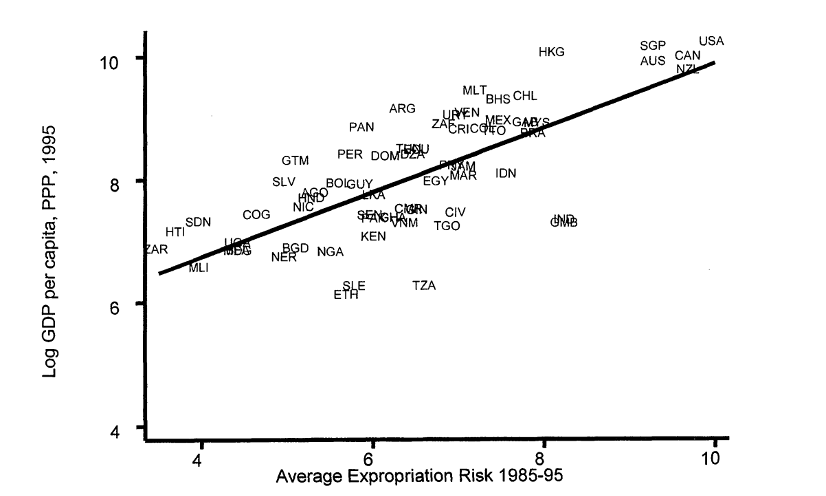
\includegraphics{Picture1.png}
\end{frame}

\begin{frame}{Institutions and Progress}
\protect\hypertarget{institutions-and-progress-1}{}
Estimated regression:
\[\log(\text{GDP per capita})=\alpha+\gamma\text{Institutions}+\mathbf{X}\beta+\varepsilon\]

Least squares estimation of this relationship is likely to violate the
exogeneity assumption!

\vfill

Issues:

\begin{enumerate}
\tightlist
\item
  Reverse causality
\item
  Omitted variables
\item
  Measurement error
\end{enumerate}

\vfill

Therefore OLS coefficients will be biased and inconsistent!

\vfill
\end{frame}

\begin{frame}{AJR (2001)}
\protect\hypertarget{ajr-2001}{}
We would need to find a variable \(z\), an ``instrument'', satisfying
the following conditions:

\begin{enumerate}
\item
  relevance: \(z\) is correlated with \(Institutions\);
\item
  exogeneity: \(z\) is uncorrelated with \(\varepsilon\)
\end{enumerate}

\vfill

If \(z\) satisfies these conditions, then we call it a valid instrument.

\vfill
\end{frame}

\begin{frame}{Graphical Representation}
\protect\hypertarget{graphical-representation}{}
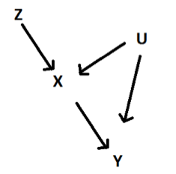
\includegraphics{Picture2.png}
\end{frame}

\begin{frame}{AJR (2001)}
\protect\hypertarget{ajr-2001-1}{}
So, how do AJR employ an IV strategy to estimate the causal effect of
institutions on economic performance?

\vfill

They focus their analysis on former European colonies and explore their
colonization as a \textbf{natural experiment}.

\vfill

Main argument:

\begin{itemize}
\tightlist
\item
  More tropical disease \(\Rightarrow\)
\item
  Less European residential settlement \(\Rightarrow\)
\item
  Worse government institutions (e.g.~less rule of law, more resource
  ``extraction'') \(\Rightarrow\) Slower long-run economic growth
\end{itemize}
\end{frame}

\begin{frame}{Main Argument}
\protect\hypertarget{main-argument}{}
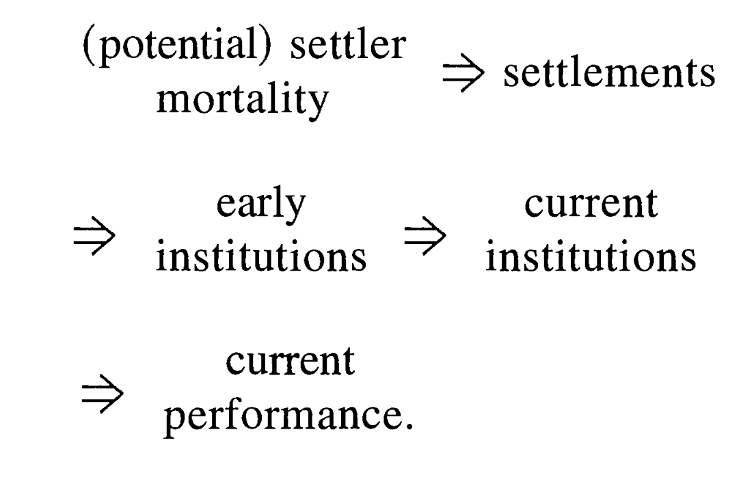
\includegraphics{Picture3.png}
\end{frame}

\begin{frame}{What makes Institutions ``extractive''?}
\protect\hypertarget{what-makes-institutions-extractive}{}
The primary role of colonies is to provide resources to the host nation:

\begin{itemize}
\tightlist
\item
  Natural resources (e.g.~lumber, coal, oil)
\item
  Finished goods (e.g.~furniture, cotton cloth)
\item
  Labor (e.g.~military services, slaves)
\end{itemize}

\vfill

In many cases, this one-way relationship can lead to policies that
sacrifice the long-term growth of the colony in favor of growth for the
host country

\vfill
\end{frame}

\begin{frame}{Extractive Institutions}
\protect\hypertarget{extractive-institutions}{}
\begin{enumerate}
\tightlist
\item
  Military administration of the colony
\item
  Indirect rule through local leaders, with no real power

  \begin{itemize}
  \tightlist
  \item
    Also, no development of robust local governance
  \end{itemize}
\item
  Investment in a select amount of infrastructure for resource
  extraction

  \begin{itemize}
  \tightlist
  \item
    Development only of the mines, port, and railroad between them
  \end{itemize}
\item
  Impressment of local population into forced labor
\item
  No political participation or rights for local population
\item
  Culture of extracting as much benefit as possible from local
  population
\end{enumerate}
\end{frame}

\begin{frame}{Inclusive Institutions}
\protect\hypertarget{inclusive-institutions}{}
Contrast this with the institutions for permanent settlement colonies:

\begin{itemize}
\tightlist
\item
  European settlers retained rights of citizenship
\item
  Well developed legal system and local governance
\item
  Strong property rights
\item
  Exemptions from certain extractive taxes and policies
\item
  Development of higher education institutions
\item
  Free movement of elites (and their rights) between colony and host
\end{itemize}
\end{frame}

\begin{frame}{Types of Colonial Settlements}
\protect\hypertarget{types-of-colonial-settlements}{}
In places with similar geography/climate to the host country, Europeans
founded permanent settlements with strong institutions - Examples: USA,
Canada, Australia, Argentina, Uruguay

\vfill

In areas with high mortality for Europeans, they didn't bother with
permanent settlements, and set up extractive frameworks instead -
Examples: Nigeria, Liberia, Andes (Peru, Bolivia), Caribbean

\vfill

Some area had both types of institutions - Examples: Apartheid South
Africa, Jim Crow Southern USA

\vfill
\end{frame}

\begin{frame}{AJR (2001)}
\protect\hypertarget{ajr-2001-2}{}
This story, if correct, allows for the use of Instrumental variables.

\vfill

Instrument they use: European settler mortality rate

\vfill

\begin{itemize}
\tightlist
\item
  Instrument Relevance: In areas with high settler mortality in the
  1700s, Europeans developed extractive institutions for those colonies
\end{itemize}

\vfill

\begin{itemize}
\tightlist
\item
  Instrument Exogeneity: Since the settler mortality rate occurred over
  200 years ago, not contemporary with any current economic performance,
  except through the present-day institutions
\end{itemize}

\vfill
\end{frame}

\begin{frame}{AJR (2001)}
\protect\hypertarget{ajr-2001-3}{}
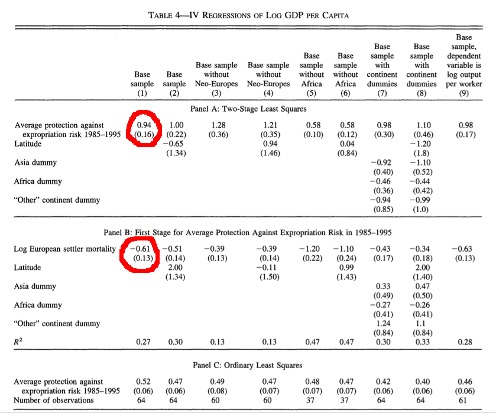
\includegraphics{Picture4jpg.jpg}
\end{frame}

\begin{frame}{Testing the IV Assumptions}
\protect\hypertarget{testing-the-iv-assumptions}{}
How can we know whether an instrument \(z\) is valid?

\vfill

Recall assumptions:

\begin{itemize}
\tightlist
\item
  Instrument Relevance (aka inclusion restriction)
\item
  Instrument Exogeneity (aka exclusion restriction)
\end{itemize}

The first assumption can easily be tested.

\begin{itemize}
\tightlist
\item
  First stage \(F\)-test tell us how strong the association between
  instrument and endogenous variable is.
\item
  Rule-of-thumb: instrument is valid if \(F\geq 10\) (maybe more).
\end{itemize}

\vfill
\end{frame}

\begin{frame}{Testing the IV Assumptions}
\protect\hypertarget{testing-the-iv-assumptions-1}{}
How about the second assumption? - This is a lot more difficult!

\vfill

We cannot directly test whether \(z\) and \(y\) are related only through
\(Institutions\).

\vfill

Usually, finding valid instruments are difficult because of the lack of
sufficient evidence to make sure the exogeneity assumption holds.

\vfill
\end{frame}

\begin{frame}{Issues with AJR's Instrument}
\protect\hypertarget{issues-with-ajrs-instrument}{}
Is settler's mortality a good instrument? - First stage \(F\)-test:
29.80

\vfill

How about the instrument Exogeneity assumption?

\vfill

Can you think about any reason for why this instrument might not satisfy
this assumption? - One potential reason: geography might affect both
historic mortality rates and present-day economic output.

\vfill
\end{frame}

\hypertarget{two-stage-least-squares}{%
\subsection{Two-Stage Least Squares}\label{two-stage-least-squares}}

\begin{frame}{Two-Stage Least Squares}
In the typical application, there is one instrument for a single
endogenous variable in the equation.

\vfill

However, the model specification may imply additional instruments.

\vfill

Let's discuss this situation in the context of simultaneous equations.
Consider the model below:

\[\text{Supply function: } q=\alpha_1p+\beta_1z_1+\varepsilon_1\]

\[\text{Demand function: } q=\alpha_2p+\beta_2 z_2+\varepsilon_2\]
\vfill

Without the inclusion of \(z_1\) and \(z_2\) in the model, there is no
way to tell which equation is the supply and which equation is the
demand (an identification problem).

\vfill
\end{frame}

\begin{frame}{Two-Stage Least Squares}
\protect\hypertarget{two-stage-least-squares-1}{}
In equilibrium, \(q^s=q^d\):

\vfill

\[\alpha_1p+\beta_1z_1+\varepsilon_1=\alpha_2p+\beta_2 z_2+\varepsilon_2\]
\[p=-\frac{\beta_1}{\alpha_1-\alpha_2}z_1+\frac{\beta_2}{\alpha_1-\alpha_2}z_2+\frac{\varepsilon_2-\varepsilon_1}{\alpha_1-\alpha_2}\]

\[p=\pi_{p1}z_1+\pi_{p2}z_2+u_p\]

\vfill

If we are interested, for example, in estimating the supply equation, we
can show that \(cov(p,\varepsilon_1)\neq 0\), violating \textbf{A.3}.

\vfill

The same reasoning can be applied to reveal that the demand equation
suffers from endogeneity as well.

\vfill
\end{frame}

\begin{frame}{Simultaneous Equations}
\protect\hypertarget{simultaneous-equations}{}
Let us discuss here what the identification problem is when we consider
a demand and supply model where there are no demand/supply shifters,
i.e.~consider:

\[\text{Supply function } q=\alpha_0+\alpha_1p+\varepsilon_1\]

\[\text{Demand function } q=\beta_0+\beta_1p+\varepsilon_2\] where
\((\varepsilon_1,\varepsilon_2)\) are \(i.i.d.\). error terms with zero
mean.

\vfill

In this model the only observable variables are quantity (\(q\)) and
prices (\(p\)), and we need to recognize that this data is only
informative about the equilibrium price and quantity \((\pi_p,\pi_q)\).
\end{frame}

\begin{frame}{Simultaneous Equations}
\protect\hypertarget{simultaneous-equations-1}{}
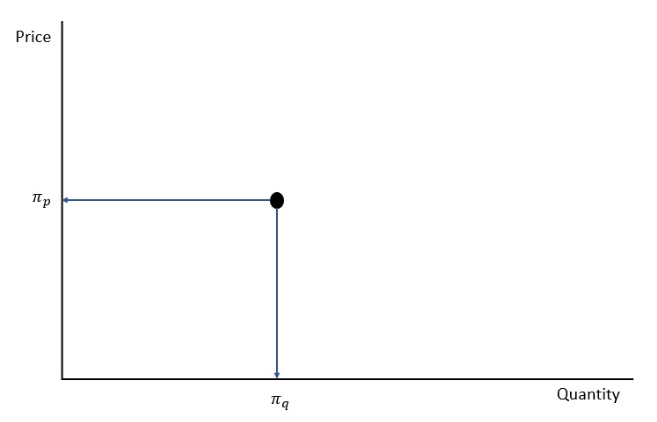
\includegraphics[width=0.7\textwidth,height=\textheight]{Picture_5.png}

\vfill

The data is not informative about the slope (intercept) of the demand
and supply equation.
\end{frame}

\begin{frame}{Simultaneous Equations}
\protect\hypertarget{simultaneous-equations-2}{}
Next, let us discuss what the identification problem is when we consider
a demand and supply model where we only have a supply shifter,
i.e.~consider:

\[\text{Supply function } q=\alpha_0+\alpha_1p+\alpha_2z+\varepsilon_1\]

\[\text{Demand function } q=\beta_0+\beta_1p+\varepsilon_2\] where
\((\varepsilon_1,\varepsilon_2)\) are \(i.i.d.\). error terms with zero
mean and \(z\) is an exogenous supply shifter.

\vfill

Do we also have an \textbf{identification problem here}?

\vfill

Here the data is informative about the equilibrium price and quantity
for different values for \(z\). Since the demand function does not
depend on the supply shifter, this permits us to identify (trace out)
the demand equation.

\vfill
\end{frame}

\begin{frame}{Simultaneous Equations}
\protect\hypertarget{simultaneous-equations-3}{}
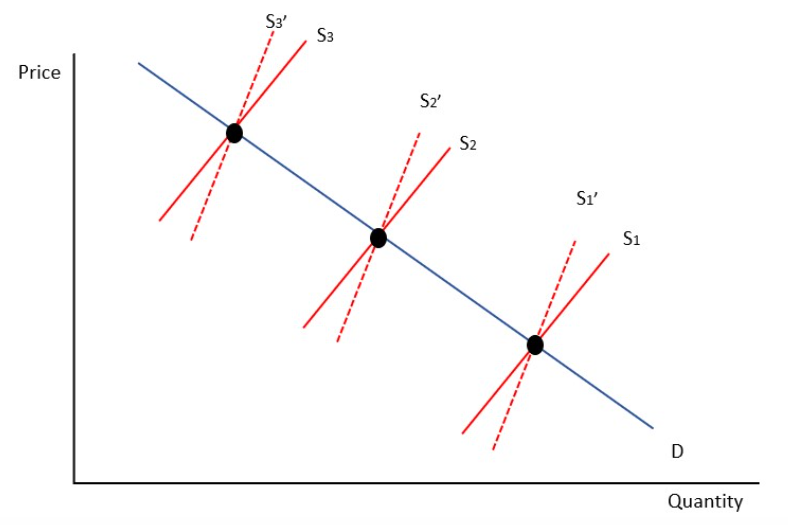
\includegraphics[width=0.6\textwidth,height=\textheight]{Picture_6.png}

\vfill

We cannot identify the supply equation as there are many supply
functions (say \(S\) and \(S'\)) that we cannot distinguish given the
observable data. Note: the slope of the supply function stays the same
when \(z\) changes.

\vfill
\end{frame}

\begin{frame}{Two-Stage Least Squares}
\protect\hypertarget{two-stage-least-squares-2}{}
Consider now an application, in an agricultural market:

\[Q_D=\alpha_0+\alpha_1 P + \alpha_2 I + \varepsilon_D\]
\[Q_S=\beta_0+\beta_1 P + \beta_2 \text{Input Price} + \beta_3\text{Rainfall} + \varepsilon_D\]
\vfill

In this model, \(Q\) and \(P\) are simultaneously determined.

\vfill

Given the approach that we have been discussing, it would appear that
the researcher could simply choose either of the two exogenous variables
(instruments) in the supply equation for identifying the demand
function.

\vfill
\end{frame}

\begin{frame}{Two-Stage Least Squares}
\protect\hypertarget{two-stage-least-squares-3}{}
However, choosing one and not using the other seems wasting valuable
information.

\vfill

It would be preferable to use the full matrix \(\mathbf{Z}\), even when
\(L>K\).

\vfill

The method of Two-Stage Least Squares (2SLS or TSLS) can be applied to
deal with this situation.

\vfill
\end{frame}

\begin{frame}{Two-Stage Least Squares}
\protect\hypertarget{two-stage-least-squares-4}{}
For the case of \(L=K\), we say the parameters are \textbf{exactly
identified}.

\vfill

For the case of \(L>K\), we say the parameters are
\textbf{overidentified}.

\vfill

If both \(\mathbf{z}_1\) and \(\mathbf{z}_2\) are exogenous and
relevant, then any linear combination of them,
\(\mathbf{z}_*=\alpha_1\mathbf{z}_1+\alpha_2\mathbf{z}_2\) would also be
a valid instrument.

\vfill
\end{frame}

\begin{frame}{Two-Stage Least Squares}
\protect\hypertarget{two-stage-least-squares-5}{}
If \(\mathbf{Z}\) contains more variables than \(\mathbf{X}\), then
\(\mathbf{Z'X}\) will be \(L\times K\) with rank \(K<L\) and will not
have an inverse.

\begin{itemize}
\tightlist
\item
  That means we cannot use \(\mathbf{b}_{IV}\).
\end{itemize}

\vfill

A choice that allows for using all of the instruments is the projection
of the columns of \(\mathbf{X}\) in the column space of \(\mathbf{Z}\),

\[\hat{\mathbf{X}}=\mathbf{Z}(\mathbf{Z'Z})^{-1}\mathbf{Z}'\mathbf{X}=\mathbf{ZF}\]

\vfill

The instruments in this case are linear combinations of the variables
(columns) in \(\mathbf{Z}\). With this choice of IV, we have

\[\mathbf{b}_{2SLS}=(\hat{\mathbf{X}}\mathbf{X}')^{-1}\hat{\mathbf{X}}'\mathbf{y}=[\mathbf{X'Z}(\mathbf{Z'Z})^{-1}\mathbf{Z}'\mathbf{X}]^{-1}\mathbf{X'Z}(\mathbf{Z'Z})^{-1}\mathbf{Z'y}\]
\end{frame}

\begin{frame}{Two-Stage Least Squares}
\protect\hypertarget{two-stage-least-squares-6}{}
Of all the different linear combinations of \(\mathbf{Z}\) that we might
choose, \(\hat{\mathbf{X}}\) is the most efficient in the sense that the
asymptotic covariance matrix of an IV estimator based on a linear
combination \(\mathbf{ZF}\) is smaller when
\(\mathbf{F}=(\mathbf{Z'Z})^{-1}\mathbf{Z'y}\) than any other
\(\mathbf{F}\) that uses all columns of \(\mathbf{Z}\).

\vfill
\end{frame}

\begin{frame}{Two-Stage Least Squares}
\protect\hypertarget{two-stage-least-squares-7}{}
This suggests that \(\mathbf{b}_{2SLS}\) can be computed in two steps:

\begin{enumerate}
\tightlist
\item
  computing \(\hat{\mathbf{X}}\) from the regression of the columns of
  \(\mathbf{X}\) on \(\mathbf{Z}\)
\item
  LS regression of \(\mathbf{y}\) on \(\hat{\mathbf{X}}\)
\end{enumerate}

\vfill

Note: The estimator
\(s^2_{IV}=\frac{\sum{(y_i-\mathbf{x}_i'\mathbf{b}_{IV})^2}}{n}\) is
inconsistent for \(\sigma^2\) with or without a correction for degrees
of freedom

\vfill
\end{frame}

\hypertarget{endogenous-dummy-variables-estimating-treatment-effects}{%
\subsection{Endogenous Dummy Variables: Estimating Treatment
Effects}\label{endogenous-dummy-variables-estimating-treatment-effects}}

\begin{frame}{Endogenous Dummy Variables: Estimating Treatment Effects}
Consider the linear regression model with a treatment dummy variable:
\[\mathbf{y}=\mathbf{x'\beta}+\delta C + \mathbf{\varepsilon}\]

The objective is to find the \textbf{treatment effect on the treated}:

\begin{itemize}
\tightlist
\item
  What is the effect of going to college on those who go to college?
\item
  What is the effect of an agricultural extension program on those who
  take part on the program?
\end{itemize}

\vfill

Complications:

\begin{enumerate}
\tightlist
\item
  Endogeneity of treatment
\item
  Missing counterfactual
\end{enumerate}

\vfill
\end{frame}

\begin{frame}{Rubin's Causal Model (1974, 1978)}
\protect\hypertarget{rubins-causal-model-1974-1978}{}
Every individual has a potential outcome, \(y\), and can be exposed to
the treatment, \(C\), which is assumed to be binary.

\vfill

Potential outcomes:

\begin{itemize}
\tightlist
\item
  \(y_1=y|(C=1)\)
\item
  \(y_0=y|(C=0)\)
\end{itemize}

\vfill

Combining these: \[y=C y_1 + (1-C)y_0=y_0+ C(y_1 - y_0)\]

The \textbf{average treatment effect} (ATE), averaged across the entire
population, is \[ATE=E[y_1-y_0]\]

\vfill
\end{frame}

\begin{frame}{Rubin's Causal Model (1974, 1978)}
\protect\hypertarget{rubins-causal-model-1974-1978-1}{}
We cannot estimate ATE because of the \emph{missing counterfactual}.

\vfill

What we would like to observe is the \textbf{average treatment effect on
the treated} (ATET):

\[ATET=E[y_1-y_0|C=1]\]

\vfill

Finding the above is one of the major themes of the recent empirical
research.

\vfill
\end{frame}

\begin{frame}{Rubin's Causal Model (1974, 1978)}
\protect\hypertarget{rubins-causal-model-1974-1978-2}{}
Let's lay out the assumptions that are relevant for such endeavor. For
doing that, consider \(\mathbf{x}\) as the exogenous information that
will be brought to bear on this estimation problem.

\vfill

\begin{enumerate}
\tightlist
\item
  \textbf{Conditional independence assumption} (CIA): Receiving the
  treatment \(C\) does not depend on the outcome variable once the
  effect of \(\mathbf{x}\) on the outcome is accounted for. In a
  regression framework, \(E[y_0|\mathbf{x},C]=E[y_0|\mathbf{x}]\) and
  \(E[y_1|\mathbf{x},C]=E[y_1|\mathbf{x}]\)
\item
  \textbf{Distribution of potential outcomes}: The model that is used
  for the outcomes in the same for treated and non-treated,
  \(f(\mathbf{y}|\mathbf{x},C=1)=f(\mathbf{y}|\mathbf{x},C=0)\)
\item
  \textbf{Stable unit treatment value assumption} (SUTVA): The treatment
  of individual \(i\) does not affect the outcome of any other
  individual, \(j\)
\item
  \textbf{Overlap assumption}: For any value of \(\mathbf{x}\),
  \(0<Prob(C=1|\mathbf{x})<1\). The population will contain a mix of
  treated and non-treted individuals.
\end{enumerate}

\vfill
\end{frame}

\begin{frame}{Regression Analysis of Treatment Effects}
\protect\hypertarget{regression-analysis-of-treatment-effects}{}
Consider an earnings equation that aims at estimating the value of a
college education:

\[\ln Earnings_i = \mathbf{x}_i'\beta+\delta C + \varepsilon_i\]

The question is: Does \(\delta\) measure the value of a college degree?

\begin{itemize}
\tightlist
\item
  The answer is no, if the typical individual who chooses to go to
  college would have relatively higher wage whether or not he or she
  went to college.
\end{itemize}

\vfill
\end{frame}

\begin{frame}{Instrumental Variables Estimation}
\protect\hypertarget{instrumental-variables-estimation-1}{}
The starting point is the Rubin's Causal Model (RCM):

\[y=\mu_0+C(\mu_1-\mu_0)+\varepsilon_0+C(\varepsilon_1-\varepsilon_0),\]
where \(\mu_j=E[y_j]\).

\vfill

Let's suppose \(\varepsilon_1=\varepsilon_0\). Then, we have

\[y=\mu_0+C(\mu_1-\mu_0)+\varepsilon_0\]

Suppose as well that there exists \(\mathbf{z}\) that contains at least
one variable that is not in \(\mathbf{x}\), such that
\(Proj(\varepsilon_0|\mathbf{X},\mathbf{z})=Proj(\varepsilon_0|\mathbf{X})\).

\begin{itemize}
\tightlist
\item
  That is, \(\mathbf{z}\) is exogenous.
\item
  Notice that we are not requiring \(\mathbf{x}\) to be exogenous.
\end{itemize}

\vfill
\end{frame}

\begin{frame}{Instrumental Variables Estimation}
\protect\hypertarget{instrumental-variables-estimation-2}{}
Let

\[Proj(\varepsilon_0|\mathbf{X})=\gamma_0+\mathbf{x}'\gamma\]

Then,

\[\mathbf{y}=(\mu_0+\gamma_0)+\delta C +\mathbf{x}'\gamma+\mathbf{w}_0,\]

where \(\mathbf{w}_0=\varepsilon_0-(\gamma_0+\mathbf{x}'\gamma)\)

\vfill

Notice that, by construction, \(\mathbf{x}\) and \(\mathbf{w}_0\) are
independent.

\vfill
\end{frame}

\begin{frame}{Instrumental Variables Estimation}
\protect\hypertarget{instrumental-variables-estimation-3}{}
To use an IV approach, we need to certify that \(\mathbf{z}\) is a
proper instrument.

\vfill

First, we assumed \(\mathbf{z}\) is exogenous.

\vfill

The relevance assumption in terms of Projection would be
\(Proj(\mathbf{C}|\mathbf{X},\mathbf{z})\neq Proj(\mathbf{C}|\mathbf{X})\).

\vfill

The model is then

\[y=\lambda_0+\gamma C+\mathbf{x}'\gamma+\mathbf{w}_0\]

\vfill
\end{frame}

\begin{frame}{Instrumental Variables Estimation}
\protect\hypertarget{instrumental-variables-estimation-4}{}
We have that \(\mathbf{X}_i=[1, C_i,\mathbf{x_i'}]\) and
\(\mathbf{Z}_i=[1, \mathbf{z}_i,\mathbf{x_i'}]\).

\vfill

The relevance assumption holds that in the projection of \(C\) on
\(\mathbf{x}\) and \(\mathbf{z}\),

\[C=\gamma_0+\mathbf{x}'\gamma_{\mathbf{x}}+\mathbf{z}'\gamma_{\mathbf{z}}+\mathbf{w}_c,\]

\(\gamma_{\mathbf{z}}\) is not zero.

\vfill

One might observe that the understanding of the functioning of the
instrument is that its variation makes participation more (or less)
likely.

\begin{itemize}
\tightlist
\item
  The relevance of the instrument is to the probability of
  participation.
\end{itemize}

\vfill

The second stage would then involve the predicted values from the first
stage.

\vfill
\end{frame}

\begin{frame}{An Application: Wating for Superman}
\protect\hypertarget{an-application-wating-for-superman}{}
Many children in large urban districts leave school with poor reading
and math skills. This perpetuates poverty and increases inequality

\vfill

Charter schools--privately managed public schools--offer a possible
solution.

\begin{itemize}
\tightlist
\item
  The Knowledge is Power Program (KIPP) is iconic in the charter
  universe, serving mostly urban minority students.
\item
  KIPP's ``No Excuses'' charter recipe includes a long school day and
  year, data-driven instruction, tutoring, and emphasizes discipline and
  comportment.
\end{itemize}

\vfill

KIPP students tend to do better than other students in the district they
hail from. But is this a causal effect?

\vfill
\end{frame}

\begin{frame}{An Application: Wating for Superman}
\protect\hypertarget{an-application-wating-for-superman-1}{}
Here's what the critics say:

\vfill

``KIPP students, as a group, enter KIPP with substantially higher
achievement than the typical achievement of schools from which they
came. . . . {[}T{]}eachers told us either that they referred students
who were more able than their peers, or that the most motivated and
educationally sophisticated parents were those likely to take the
initiative . . . and enroll in KIPP.''

\vfill
\end{frame}

\begin{frame}{The Superman selection story}
\protect\hypertarget{the-superman-selection-story}{}
Let \(C_i\) denote attendance at KIPP and \(y_i\) be an achievement test
outcome.

\vfill

Under constant causal effects,

\[y=C y_1 + (1-C)y_0=y_0+ C(y_1 - y_0)=\alpha+\gamma C+\varepsilon\]

\vfill

Even adding exogenous controls \(\mathbf{x}\), the CIA assumption is
likely to be violated (why?).

\vfill
\end{frame}

\begin{frame}{Defining Instruments}
\protect\hypertarget{defining-instruments}{}
An instrument (\(z_i\)) for KIPP attendance is correlated with \(C_i\)
but uncorrelated with \(\varepsilon_{i}\).

\vfill

In the present context, instrumental variable \(z_i\) is assumed to
satisfy:

\begin{enumerate}
\tightlist
\item
  \(Cov(z_i, C_i)\neq0\)
\item
  \(Cov(z_i, \varepsilon_i)=0\)
\end{enumerate}

In the simple regression case,

\[\delta_{IV}=\frac{Cov(y,z)}{Cov(C,z)}\]

\vfill

We can multiply the above by \(Var(z)/Var(z)\) to get

\[\delta_{IV}=\frac{\text{Reduced form}}{\text{First stage}}=\frac{Cov(y,z)/Var(z)}{Cov(C,z)/Var(z)}\]

\vfill
\end{frame}

\begin{frame}{Defining Instruments}
\protect\hypertarget{defining-instruments-1}{}
Because we can solve for the causal coefficient of interest from
observable moments (in this case, variances and covariances), \(\delta\)
is said to be identified.

\vfill

Thus, the IV estimator is a ratio of regression estimates:

\[\hat{\delta}_{IV}=\frac{s_{y,z}/s^2_z}{s_{C,z}/s^2_z}\]

\vfill
\end{frame}

\begin{frame}{Playing the KIPP Lottery}
\protect\hypertarget{playing-the-kipp-lottery}{}
Like all Massachusetts charter schools, KIPP Lynn assigns seats by
lottery (i.e., at random) when over-subscribed

\vfill

In this case, instrument \(z_i\) is a dummy variable indicating the set
of KIPP applicants randomly offered a KIPP seat

\begin{itemize}
\tightlist
\item
  Because the lottery is how most KIPP applicants get seated there, the
  relevance assumption is satisfied
\item
  Because lottery offers are randomly assigned, they're likely to be
  independent of potential outcomes, satisfying the exogeneity
  assumption
\end{itemize}

\vfill
\end{frame}

\begin{frame}{Playing the KIPP Lottery}
\protect\hypertarget{playing-the-kipp-lottery-1}{}
Bernoulli (dummy) instruments generate a useful simplification of the IV
equation:

\[\delta_{IV}=\frac{Cov(y,z)/Var(z)}{Cov(C,z)/Var(z)}=\frac{E[y_i|z_i=1]-E[y_i|z_i=0]}{E[C_i|z_i=1]-E[C_i|z_i=0]}\]
We can therefore construct IV estimates using a ratio of differences in
means:

\[\hat{\delta}_{IV}=\frac{\bar{y}_1-\bar{y}_0}{\bar{C}_1-\bar{C}_0}\]

This formulation is called a \textbf{Wald estimator} after Wald (1940).

\vfill
\end{frame}

\begin{frame}{Application and enrollment data from KIPP Lynn lotteries}
\protect\hypertarget{application-and-enrollment-data-from-kipp-lynn-lotteries}{}
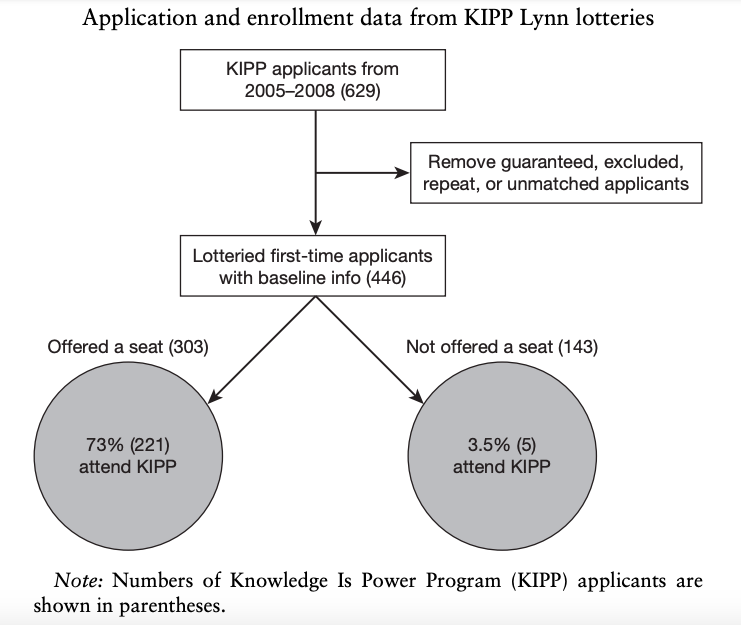
\includegraphics[width=0.6\textwidth,height=\textheight]{figure_kipp.png}
\end{frame}

\begin{frame}{Estimated Treatment Effect}
\protect\hypertarget{estimated-treatment-effect}{}
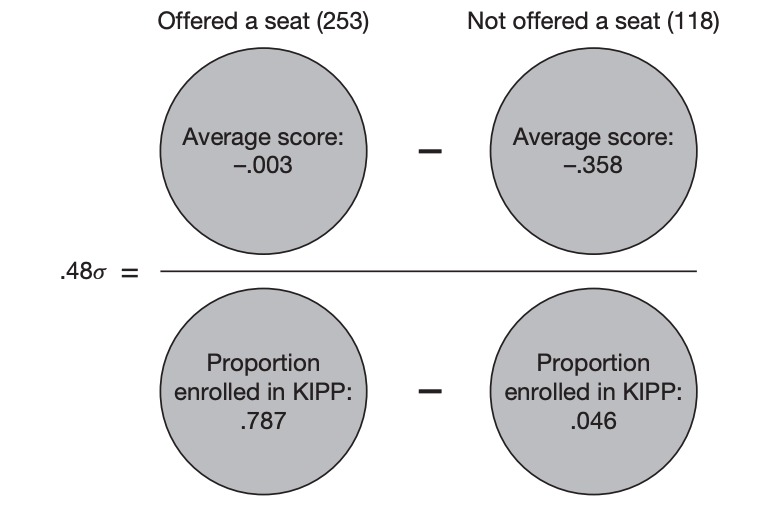
\includegraphics[width=0.6\textwidth,height=\textheight]{figure_kipp2.png}

\vfill

The effect of Knowledge Is Power Program (KIPP) enrollment described by
this figure is \(.48\sigma = .355\sigma/.741\).

\vfill
\end{frame}

\begin{frame}{IV With Heterogeneous Potential Outcomes}
\protect\hypertarget{iv-with-heterogeneous-potential-outcomes}{}
KIPP lottery offers affect KIPP enrollment for many applicants\ldots{}
but not all

\begin{itemize}
\tightlist
\item
  Some offered a seat at KIPP nevertheless go elsewhere
\item
  A few not offered a seat in the lottery manage to sneak in anyway
\end{itemize}

\vfill

How should we interpret IV estimates in light of this fact?

\vfill
\end{frame}

\begin{frame}{Additional Assumptions for the IV}
\protect\hypertarget{additional-assumptions-for-the-iv}{}
Applying IV estimation to the Rubin's model in situations like this
implies two additional assumptions regarding the instrument \(z\):

\begin{enumerate}
\tightlist
\item
  \textbf{Independence assumption}: The IV is independent of the vector
  of potential outcomes and potential treatment assignments (i.e.~``as
  good as randomly assigned'')
\item
  \textbf{Monotonicity} The instrumental variable (weakly) operates in
  the same direction on all individual units. In other words, while the
  instrument may have no effect on some people, all those who are
  affected are affected in the same direction (i.e., positively or
  negatively, but not both).
\end{enumerate}

\vfill
\end{frame}

\begin{frame}{IV With Heterogeneous Potential Outcomes}
\protect\hypertarget{iv-with-heterogeneous-potential-outcomes-1}{}
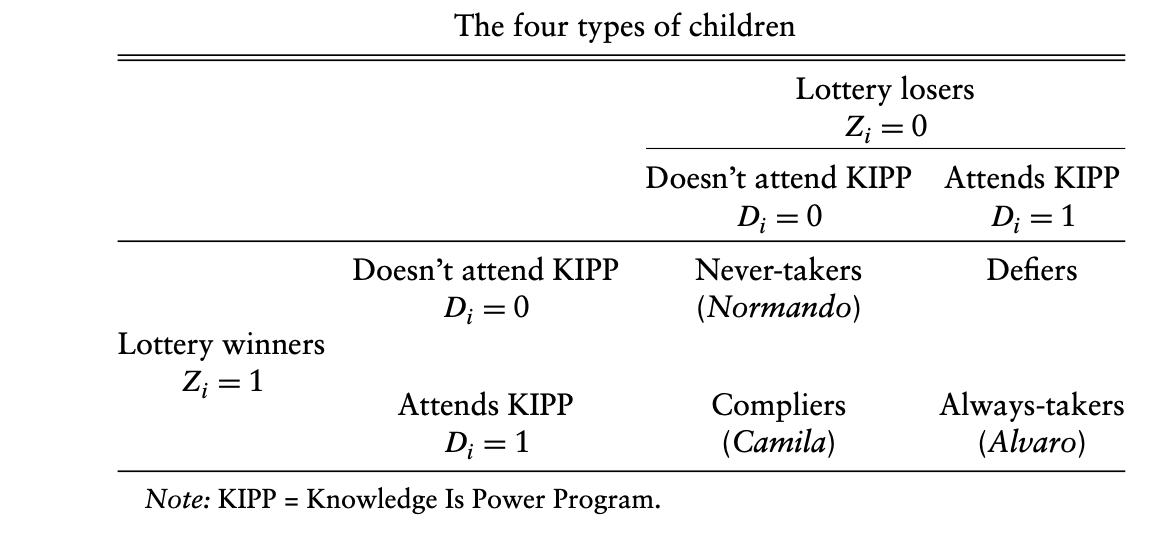
\includegraphics[width=0.6\textwidth,height=\textheight]{figure_kipp3.png}

\vfill

There are are only three in this case: no defiers allowed!

\vfill
\end{frame}

\begin{frame}{IV With Heterogeneous Potential Outcomes}
\protect\hypertarget{iv-with-heterogeneous-potential-outcomes-2}{}
In a world of heterogeneous potential outcomes,

\[\delta_{IV}=\frac{E[y_i|z_i=1]-E[y_i|z_i=0]}{E[C_i|z_i=1]-E[C_i|z_i=0]}=E[y_{1i}-y_{0i}|\text{Complier}]\]

\vfill

The parameter \(E[y_{1i}-y_{0i}|\text{Complier}]\) is called a
\textbf{local average treatment effect} (LATE).

\vfill

In general, LATE differs from the effect of treatment on the treated,
\(E[y_{1i}-y_{0i}|C_i = 1]\), because some treated are always-takers,
like Alvaro.

\vfill

With few always-takers (as in the KIPP lottery), we expect
\(E[y_{1i}-y_{0i}|\text{Complier}]\approx E[y_{1i}-y_{0i} |C_i=1]\).

\vfill
\end{frame}

\begin{frame}{IV With Heterogeneous Potential Outcomes}
\protect\hypertarget{iv-with-heterogeneous-potential-outcomes-3}{}
The LATE parameters is the average causal effect of \(C\) on \(y\) for
those whose treatment status was changed by the instrument, \(z\).

-These are the compliers!

\vfill

We have reviewed the properties of IV with heterogeneous treatment
effects using a very simple dummy endogenous variable, dummy IV, and no
additional controls example.

\vfill

The intuition of LATE generalizes to most cases where we have continuous
endogenous variables and instruments, and additional control variables

\vfill
\end{frame}

\begin{frame}{What Does IV (Not) Estimate?}
\protect\hypertarget{what-does-iv-not-estimate}{}
IV estimates the average treatment effect for compliers, or LATE

\vfill

Without further assumptions (e.g., constant causal effects), LATE is not
informative about effects on never-takers or always-takers because the
instrument does not affect their treatment status

\vfill

So what? Well, it matters because in most applications, we would be
mostly interested in estimating the average treatment effect on the
treated.

\vfill

But that's not usually possible with IV.

\vfill
\end{frame}

\begin{frame}{The LATE Cup}
\protect\hypertarget{the-late-cup}{}
Different applied econometricians have different views on LATE:

\begin{itemize}
\item
  Heckman, Deaton, and others: The LATE cup is half empty (or all
  empty!): We don't get what we want, the average treatment effect on
  the treated, so IV is somewhat useless, and we need to augment it with
  something else to produce economically meaningful parameters
  (e.g.~more structural econometric models).
\item
  Angrist, Imbens, and others: The LATE cup is half full. We don't get
  the average effect on a stable population (like the average treatment
  effect on the treated) but we get something that still makes some
  sense (particularly for policy).
\end{itemize}

\vfill
\end{frame}

\hypertarget{hypothesis-tests}{%
\subsection{Hypothesis Tests}\label{hypothesis-tests}}

\begin{frame}{Hypothesis Tests}
Let's now discuss the issue of hypothesis testing in the world of
instrumental variables.

We will detail:

\begin{enumerate}
\tightlist
\item
  Testing restrictions
\item
  Specification tests
\end{enumerate}
\end{frame}

\begin{frame}{Testing Restrictions}
\protect\hypertarget{testing-restrictions}{}
For testing linear restrictions in \(H_0: \mathbf{R\beta}=\mathbf{q}\),
the test statistic would be

\[\chi^2[J]=(\mathbf{R\hat{\beta}}-\mathbf{q})'[\mathbf{R}Est.Asy.Var(\hat{\beta})\mathbf{R}']^{-1}(\mathbf{R\hat{\beta}}-\mathbf{q})\]
For a simple hypothesis that a coefficient equals zero, this is the
square of the usual \(t\) ratio.

\vfill
\end{frame}

\begin{frame}{Testing Restrictions}
\protect\hypertarget{testing-restrictions-1}{}
For the 2SLS estimator based on least squares regression of
\(\mathbf{y}\) on \(\mathbf{X}\), an asymptotic \(F\) statistic can be
computed:

\[F[J,n-K]=\frac{\{\sum{(\mathbf{y}_i-\hat{\mathbf{x}}_i'\hat{\beta}_{restricted})^2}-\sum{(\mathbf{y}_i-\hat{\mathbf{x}}_i'\hat{\beta}_{unrestricted})^2} \}/J}{\sum{(\mathbf{y}_i-\hat{\mathbf{x}}_i'\hat{\beta}_{unrestricted})^2}/(n-K)}\]

\vfill
\end{frame}

\begin{frame}{Specification Tests}
\protect\hypertarget{specification-tests}{}
In comparing \(\mathbf{b}_{LS}\) and \(\mathbf{b}_{IV}\), we see that
\(\mathbf{b}_{LS}\) is unambiguously more efficient.

\vfill

The difference between the asymptotic covariance matrices of the two
estimators is

\[Asy.Var[\mathbf{b}_{IV}] - Asy.Var[\mathbf{b}_{LS}]=\frac{\sigma^2}{n}\text{plim }n\{[\mathbf{X'X}-\mathbf{X'M_ZX}]^{-1}-[\mathbf{X'X}]^{-1}\}\]

\vfill

The matrix in braces is nonnegative definite, which establishes that
least squares is more efficient than IV.

\vfill
\end{frame}

\begin{frame}{Specification Tests}
\protect\hypertarget{specification-tests-1}{}
However, \(\mathbf{b}_{IV}\) is robust, as it is consistent whether or
not \(\text{plim }(\mathbf{X'\varepsilon}/n)=0\).

\vfill

If the condition above holds (that is, \(\gamma=0\)), then IV is not
needed so \(\mathbf{b}_{IV}\) would be preferable.

\vfill

We will thus, devise tests about two aspects:

\begin{enumerate}
\tightlist
\item
  a test that reveals the bias of the least squares
\item
  a test for overidentification for the case of 2SLS
\end{enumerate}

\vfill
\end{frame}

\begin{frame}{Testing for Endogeneity: The Hausman and Wu Specification
Tests}
\protect\hypertarget{testing-for-endogeneity-the-hausman-and-wu-specification-tests}{}
Consider a comparison of the covariance matrices of \(\mathbf{b}_{LS}\)
and \(\mathbf{b}_{IV}\) under the hypothesis that both estimators are
consistent (\(\text{plim }(\mathbf{X'\varepsilon}/n)=0\)).

\vfill

The problem in estimating the empirical counterpart is that
\(\text{plim }(\mathbf{X'e}/n)=0\) by construction.

\vfill

Hausman (1978) developed an alternative strategy. Under \(H_0\), both
\(\mathbf{b}_{IV}\) and \(\mathbf{b}_{LS}\) are consistent estimators of
\(\beta\).

\vfill

The suggestion is then to examine
\(\mathbf{d}=\mathbf{b}_{IV}-\mathbf{b}_{LS}\).

\vfill
\end{frame}

\begin{frame}{The Hausman (1978) Test}
\protect\hypertarget{the-hausman-1978-test}{}
Under \(H_0\), \(\text{plim }\mathbf{d}=\mathbf{0}\) whereas under
\(H_1\), \(\text{plim }\mathbf{d}\neq\mathbf{0}\)

\vfill

We test this hypothesis with a Wald statistic:

\[\begin{split}\mathbf{H} & =\mathbf{d}'\{Est.Asy.Var(\mathbf{d})\}^{-1}\mathbf{d}\\
& = (\mathbf{b}_{IV}-\mathbf{b}_{LS})'\{Est.Asy.Var(\mathbf{b}_{IV})-Est.Asy.Var(\mathbf{b}_{LS})\}^{-1}(\mathbf{b}_{IV}-\mathbf{b}_{LS})\\
& = (\mathbf{b}_{IV}-\mathbf{b}_{LS})'\hat{\mathbf{H}}^{-1}(\mathbf{b}_{IV}-\mathbf{b}_{LS})\end{split}\]

where \(\hat{\mathbf{H}}^{-1}\) is the estimator of
\(\{Est.Asy.Var(\mathbf{b}_{IV})-Est.Asy.Var(\mathbf{b}_{LS})\}^{-1}\),
\(\sigma^2 \{[\mathbf{X'X}-\mathbf{X'M_ZX}]^{-1}-[\mathbf{X'X}]^{-1}\}^{-1}\).

\vfill
\end{frame}

\begin{frame}{The Hausman (1978) Test}
\protect\hypertarget{the-hausman-1978-test-1}{}
Under \(H_0\), we have two different, but consistent estimators of
\(\sigma^2\).

\vfill

If we use \(s^2\) as the common estimator, we have

\[\mathbf{H}=\frac{\mathbf{d}'[(\hat{\mathbf{X}}'\hat{\mathbf{X}})^{-1}-(\mathbf{X'X})^{-1}]^{-1}\mathbf{d}}{s^2}\]

\vfill

The degrees of freedom of this chi-squared distributed variable is
\(K^*=K-K_0\), where \(K_0\) is the number of exogenous variables in
\(\mathbf{X}\)

\vfill

The Wald test requires a generalized inverse {[}done in Hausman and
taylor (1981){]}, and it is a bit cumbersome.

\vfill
\end{frame}

\begin{frame}{The Wu (1973) Test}
\protect\hypertarget{the-wu-1973-test}{}
An alternative \textbf{variable addition test} approach was devised by
Wu (1973) and Durbin (1954).

\vfill

An \(F\) statistic with \(K^*\) and \(n-K-K^*\) degrees of freedom can
be used to test the joint significance of the elements of \(\gamma\) in
the augmented regression

\[\mathbf{y}=\mathbf{X\beta}+\hat{\mathbf{X}^*\gamma}+\varepsilon^*,\]

where \(\hat{\mathbf{X}}^*\) are the fitted values in the regression of
the variables in \(\mathbf{X}^*\) on \(\mathbf{Z}\).

\vfill
\end{frame}

\begin{frame}{A Test for Overidentification}
\protect\hypertarget{a-test-for-overidentification}{}
A couple of points for consideration:

\begin{itemize}
\tightlist
\item
  The motivation for choosing IV is consistency, and not efficiency.
\item
  2SLS represents the most efficient use of all \(L\) instruments.
\end{itemize}

\vfill

The IV is developed around the \textbf{orthogonality conditions}

\[E[\mathbf{z}_i\varepsilon_i]=0\]

The sample counterpart to this is the moment equation

\[\frac{1}{n}\sum{\mathbf{z}_ie_i}=0\]

\vfill
\end{frame}

\begin{frame}{A Test for Overidentification}
\protect\hypertarget{a-test-for-overidentification-1}{}
When \(L>K\), we can consider the additional restrictions as a
hypothesis that might or might not be supported by the
overidentification of the model.

\vfill

When \(L=K\), the system is exactly identified and there is only one
solution to \(\frac{1}{n}\sum{\mathbf{z}_ie_i}=0\).

\vfill

When \(L>K\), the above sum does not need to equal zero. We can, then
devise a test for the additional instruments for overidentification.

\vfill
\end{frame}

\begin{frame}{A Test for Overidentification}
\protect\hypertarget{a-test-for-overidentification-2}{}
The test statistic will be a Wald statistic. The sample moment is

\[\bar{\mathbf{m}}=\frac{1}{n}\sum{\mathbf{z}_ie_{IV,i}}=\frac{1}{n}\sum{\mathbf{z}_i(\mathbf{y}_i-\mathbf{x}_i'\mathbf{b}_{IV})}\]

The Wald statistic is

\[\chi^2[L-K]=\bar{\mathbf{m}}'[Var(\bar{\mathbf{m}})]^{-1}\bar{\mathbf{m}}\]

If the equation is exactly identified, then
\((1/n)\mathbf{Z}'\mathbf{e}_{IV}\) will be exactly zero.

\vfill

The variance \(Var(\bar{\mathbf{m}})\) can be computed by
\(\frac{\sigma^2}{n^2}\mathbf{Z'Z}\), and we can use the sample
estimator of \(\sigma^2\) to estimate it.

\vfill

One important limitation of the test is that it suggests only that one
or more than one of the elements in the orthogonality conditions are
nonzero. It does not tell us which elements in particular are those.

\vfill
\end{frame}

\begin{frame}{Weak Instruments}
\protect\hypertarget{weak-instruments}{}
So far, we have focused on the exogeneity assumption.

\vfill

Let's now consider the relevance assumption:
\(\text{plim }(1/n)\mathbf{Z'X}=\mathbf{Q}_{ZX}\), a finite, nonzero,
\(L\times K\) matrix with rank \(K\).

\vfill

We say instruments are \emph{weak} when they are only slightly
correlated with the \(\mathbf{X}\).

\begin{itemize}
\tightlist
\item
  That is, \(\text{plim }(1/n)\mathbf{Z'X}\) is \emph{close} to zero.
\end{itemize}

\vfill
\end{frame}

\begin{frame}{Weak Instruments}
\protect\hypertarget{weak-instruments-1}{}
Superficially, the problem of weak instruments shows up in the
asymptotic covariance matrix of the IV estimator:

\[Asy.Var[\mathbf{b}_{IV}]=\frac{\sigma_{\varepsilon}^2}{n}\left(\frac{\mathbf{Z'X}}{n}\right)^{-1}\left(\frac{\mathbf{Z'Z}}{n}\right)\left(\frac{\mathbf{X'Z}}{n}\right)^{-1}\]

which will be large when the instruments are weak.

\vfill
\end{frame}

\begin{frame}{Weak Instruments}
\protect\hypertarget{weak-instruments-2}{}
However, the problem goes beyond precision of the estimates. A recent
literature has been shown that

\begin{enumerate}
\tightlist
\item
  The 2SLS estimator is badly biased toward the OLS estimator, which is
  inconsistent.
\item
  The standard asymptotics will not give an accurate framework for
  statistical inference.
\end{enumerate}

\vfill
\end{frame}

\begin{frame}{Weak Instruments}
\protect\hypertarget{weak-instruments-3}{}
To detect weak instruments, the standard practice (for the case of a
single endogenous variable) is to evaluate the \(F\) statistic for
testing the hypothesis that all coefficients in the regression
\[\mathbf{x}_i=\mathbf{z}_i'\pi + u_i\] are all zero.

\vfill

An \(F\) statistic less than 10 signals the problem.

\vfill
\end{frame}

\begin{frame}{Weak Instruments}
\protect\hypertarget{weak-instruments-4}{}
For the general case, Godfrey (1999) proposes a statistic which is the
ratio of the variances of the two estimates, 2SLS and OLS:

\[R_k^2=\frac{(\mathbf{X'X})^{kk}}{(\mathbf{\hat{X}'\hat{\mathbf{X}}})^{kk}}\]
where the superscript indicates the element of the inverse matrix.

The \(F\) statistic can then be based on this measure:

\[F=\frac{R^2_k/(L-1)}{(1-R_k^2)/(n-L)}\] assuming that \(\mathbf{Z}\)
contains a constant term.

\vfill
\end{frame}

\begin{frame}{Weak Instruments}
\protect\hypertarget{weak-instruments-5}{}
The natural recourse in the face of weak instruments is to drop the
endogenous variable from the model or improve the instrument set.

\vfill

Each of these is a specification issue. Strictly in terms of estimation
strategy within the framework of the data and specification in hand,
there is scope for OLS to be the preferred strategy.

\vfill
\end{frame}

\hypertarget{measurement-error}{%
\subsection{Measurement Error}\label{measurement-error}}

\begin{frame}{Measurement Error}
We have assumed so far that all variables are true measurements of their
theoretical counterparts.

\vfill

For example, we have assumed that we can perfectly capture the level of
education from the data (with measures such as number of years of
schooling) but it might be challenging to truly quantify it.

\vfill
\end{frame}

\begin{frame}{Least Squares Attenuation}
\protect\hypertarget{least-squares-attenuation}{}
Let's focus on the rather simplistic case of a model with a single
regressor (and no constant):

\[y^*=\beta x^*+\varepsilon\]

where all classical assumptions hold.

\vfill

Suppose that the observed data are only imperfectly measured versions of
\(y^*\) and \(x^*\):

\[y=y^*+\nu \text{ with }\nu \sim N[0,\sigma_{\nu}^2]\]

\[x=x^*+u \text{ with } u \sim N[0,\sigma_u^2]\] Assume as well that
\(\nu\) and \(u\) are independent of each other and of \(x^*\) and
\(y^*\).

\vfill
\end{frame}

\begin{frame}{Least Squares Attenuation}
\protect\hypertarget{least-squares-attenuation-1}{}
Let's start with the case in which only \(y^*\) is measured with error.
Thus,

\[y=\beta x^* + \varepsilon+\nu=\beta x^* + \varepsilon'\]

This result still conforms to the assumptions of the classical
regression model.

\begin{itemize}
\tightlist
\item
  Measurement error in the dependent variable can be absorbed by the
  disturbances.
\end{itemize}

\vfill
\end{frame}

\begin{frame}{Least Squares Attenuation}
\protect\hypertarget{least-squares-attenuation-2}{}
From now on, let's focus on the situation of measurement error problems
only in the independent variables of the model.

\vfill

Consider, then, the regression of \(y\) on \(x\):

\[y=\beta(x-u)+\varepsilon=\beta x +(\varepsilon-\beta u)=\beta x +w\]

We can find:

\[Cov[x,w]=-\beta \sigma_u^2\]

Therefore, assumption A.3. is violated and the LS estimator is
\emph{inconsistent}.

\vfill
\end{frame}

\begin{frame}{Least Squares Attenuation}
\protect\hypertarget{least-squares-attenuation-3}{}
Notice the following:

\[b=\frac{(1/n)\sum{x_i y_i}}{(1/n)\sum{x_i^2}}\]

Its probability limit is given by

\[\text{plim }b=\frac{\beta Q^*}{Q^*+\sigma_u^2}=\frac{\beta}{1+\sigma^2_u/Q^*}\]

where \(Q^*=\text{plim }(1/n)\sum{x_i^{*2}}\).

\vfill

As long as \(\sigma_u^2\) is positive, \(b\) is inconsistent, with a
persistent bias toward zero. This effect is known as
\textbf{attenuation}.

\vfill
\end{frame}

\begin{frame}{Least Squares Attenuation in Multiple Regression}
\protect\hypertarget{least-squares-attenuation-in-multiple-regression}{}
In a multiple regression model, matters only get worse.

\vfill

Measurement error in one variable can contaminate all other regressors
and render LS coefficients inefficiently estimated, even those with no
measurement error.

\vfill
\end{frame}

\begin{frame}{Instrumental Variables Estimation}
\protect\hypertarget{instrumental-variables-estimation-5}{}
Consider again the errors in variables model

\[y^*=\beta x^*+\varepsilon\]

\[y=y^*+\nu \text{ with }\nu \sim N[0,\sigma_{\nu}^2]\]

\[x=x^*+u \text{ with } u \sim N[0,\sigma_u^2]\]

Suppose now that there exists a variable \(z\) such that \(z\) is
correlated with \(x^*\) but not \(u\).

\vfill

As an example, suppose \(x\) is reported income in survey data, which is
badly reported.

\vfill
\end{frame}

\begin{frame}{Instrumental Variables Estimation}
\protect\hypertarget{instrumental-variables-estimation-6}{}
Suppose, however, that we could observe the amount of checks written by
the head(s) of the household.

\vfill

Is this a good instrument?

\begin{itemize}
\tightlist
\item
  Highly correlated with income, \(y^*\)
\item
  Not significantly related to the errors of measurement
\end{itemize}

\vfill
\end{frame}

\begin{frame}{Instrumental Variables Estimation}
\protect\hypertarget{instrumental-variables-estimation-7}{}
If these conditions are satisfied, we have

\[\text{plim }\frac{(1/n)\sum{y_i z_i}}{(1/n)\sum{x_i z_i}}=\text{plim }\frac{(1/n)\beta\sum{x_i^* z_i}}{(1/n)\sum{x_i z_i}}=\beta\frac{cov(x_i^*,z_i)}{cov(x_i^*,z_i)}=\beta\]

\vfill

For the general case,
\(\mathbf{y}=\mathbf{X^*\beta}+\mathbf{\varepsilon}\),
\(\mathbf{X}=\mathbf{X^*}+\mathbf{U}\), suppose there exists
\(\mathbf{Z}\) that is not correlated with the disturbances or the
measurement error but is correlated with the regressors, \(\mathbf{X}\).

\vfill

Then, \(\mathbf{b}_{IV}=(\mathbf{Z'X})^{-1}\mathbf{Z'y}\) is consistent
and asymptotically normally distributed with asymptotic covariance
matrix that is estimated with

\[Est.Asy.Var[\mathbf{b}_{IV}]=\hat{\sigma}^2(\mathbf{Z'X})^{-1}(\mathbf{Z'Z})(\mathbf{X'Z})^{-1}\]

\vfill
\end{frame}

\begin{frame}{Proxy Variables}
\protect\hypertarget{proxy-variables}{}
Some variables simply have no observable counterpart: Education,
ability, intelligence are examples.

\vfill

Consider a \textbf{structural model}:

\[Earnings=\beta_1+\beta_2 Experience + \beta_3 Industry + \beta_4 Ability+\varepsilon\]

Although we cannot observe ability, we can use an indicator, IQ, which
can be correlated with the unobserved variable \(Ability\):

\[IQ=\alpha_1 +\alpha_2 Ability+\nu\]
\end{frame}

\begin{frame}{Proxy Variables}
\protect\hypertarget{proxy-variables-1}{}
We can insert one equation into the other to obtain the \textbf{reduced
form} equation

\[Earnings=(\beta_1-\beta_4\alpha_1/\alpha_2)+\beta_2 Experience+\beta_3 Industry+(\beta_4/\alpha_2)IQ+(\varepsilon-\nu\beta_4/\alpha_2)\]

Notice that for us to being able to estimate this equation, we require:

\begin{enumerate}
\tightlist
\item
  \(IQ\) not be related to the other variables of the model
\item
  \(\nu\) not be related to the other variables of the model
\item
  \(E[Earnings|Experience, Industry, Ability,IQ]=E[Earnings|Experience, Industry, Ability]\)
\end{enumerate}

\vfill
\end{frame}


\section[]{}
\frame{\small \frametitle{Table of Contents}
\tableofcontents}
\end{document}
